\documentclass[12pt]{report}
\usepackage[utf8]{inputenc}
\usepackage[T1]{fontenc}
\usepackage[francais]{babel}
\usepackage{graphicx}
\usepackage{amsfonts}
\usepackage{hyperref}
\usepackage{fixltx2e}
% Packages graphiques
\usepackage{caption} 
\usepackage{tikz}
\usepackage{mathtools}
\usepackage{amsmath}
\usepackage{pgfplots}
\usetikzlibrary{plotmarks}
\pgfplotsset{compat=1.8}

\title{Voyageur du Commerce}
\author{Afanyan Marcy Phan Pindat}
\date{\today}
\begin{document}

\begin{titlepage}

\newcommand{\HRule}{\rule{\linewidth}{0.5mm}} 

\center 
 


\textsc{\LARGE Université de Bordeaux}\\[1.5cm] 
\textsc{\Large Département Informatique}\\[0.5cm] 
\textsc{\large Environnement de développement \& Projet de Programmation 1}\\[0.5cm] 

%----------------------------------------------------------------------------------------
%	TITRE
%----------------------------------------------------------------------------------------

\HRule \\[0.4cm]
{ \huge \bfseries Problème du Voyageur de Commerce}\\[0.4cm] 
\HRule \\[1.5cm]
 
%----------------------------------------------------------------------------------------
%	AUTEURS
%----------------------------------------------------------------------------------------

\begin{minipage}{0.4\textwidth}
\begin{flushleft} \large
\emph{Auteurs:}\\
David \textsc{Phan}\\
Jason \textsc{Pindat}\\
Nicolas \textsc{Marcy}\\
Raphaël \textsc{Afanyan}\\

\end{flushleft}
\end{minipage}
~
\begin{minipage}{0.4\textwidth}
\begin{flushright} \large
\emph{Encadrant:} \\
Irène \textsc{Durand} 
\end{flushright}
\end{minipage}\\[2cm]



%----------------------------------------------------------------------------------------
%	DATE 
%----------------------------------------------------------------------------------------

{\large \today}\\[1.5cm] % Date

%----------------------------------------------------------------------------------------
%	LOGO
%----------------------------------------------------------------------------------------


\includegraphics[height=80px]{bxlogo.jpg}\\[1cm] % Logo université
 
%----------------------------------------------------------------------------------------

\vfill 

\end{titlepage}





%----------------------------------------------------------------------------------------
%	SOMMAIRE 
%----------------------------------------------------------------------------------------
\tableofcontents



%----------------------------------------------------------------------------------------
%	CHAPITRE 1 INTRODUCTION 
%----------------------------------------------------------------------------------------

%1 Introduction
\chapter{Introduction}


%1.1 Présentation
\section{Présentation}
Dans le cadre de ce projet, on s'intéresse au problème classique du \textit{voyageur de commerce} qui consiste à, étant donné un ensemble de villes séparées par des distances données, trouver le \textit{cycle hamiltonien}, chemin passant par toutes les villes, une fois et une seule. Il s'agit d'un problème d'optimisation pour lequel on ne connait pas d'algorithme permettant de trouver une solution exacte en un temps polynomial bien qu'on puisse vérifier rapidement toute solution proposée, c'est un problème NP-complet. En revanche, de nombreux autres algorithmes existent afin de résoudre ce problème plus ou moins efficacement. Il nous a été demandé d'écrire au moins 4 algorithmes permettant, à partir d'un fichier TSP, de trouver une solution et d'en donner la longueur pour pouvoir la comparer avec les autres. Au total, 8 différentes versions et implémentations de ces algorithmes ont été réalisées.\\



%1.2 Notre programme
\section{Notre programme}

Notre programme répond donc au cahier des charges initial auquel nous avons ajouté d'autres options : 
\begin{itemize}
   \item un algorithme avec une heuristique simple (\textit{Nearest Neighbour}).
   \item un algorithme d'approximation (\textit{Minimum Spanning Tree}).
   \item un algorithme exact par recherche exhaustive (plusieurs versions différentes en recherchant le meilleur temps d'exécution).
   \item un algorithme exact utilisant la technique de "\textit{Branch and Bound}", et une version comprenant une relaxation avec \textit{Nearest Neighbour} et \textit{Minimum Spanning Tree}, une autre avec relaxation de \textit{Held-Karp}
   \item pouvoir charger des instances \textbf{TSPLIB} (.tsp) codées sous la forme de matrices complètes. 
   \item pouvoir retourner les solutions dans le format \textbf{TSPLIB} (.tour).
   \item effectuer des tests de performance.
   \item visualiser graphiquement la route calculée (en utilisant \textbf{DISPLAY\_DATA\_SECTION})
   \item retourner les données et traitements des instances faits par le programme dans un format générique (\textbf{JSON}).
\end{itemize}



%----------------------------------------------------------------------------------------
%   CHAPITRE 2 PROGRAMME TSP 
%----------------------------------------------------------------------------------------



%2 Le programme Traveling Salesman Problem Solver
\chapter{Le \textit{Traveling Salesman Problem Solver}}

Nous avons nommé notre programme \textit{Traveling Salesman Problem Solver}, qui est une traduction à Résolveur du Problème du Voyageur de commerce.

%2.1 Présentation des fonctionnalités
\section{Fonctionnalités}

Le programme peut s'utiliser en deux modes : le mode console, et le mode graphique.\
Les deux modes présentent les fonctionnalités suivantes : \
\begin{itemize}
	\item Ouvrir et instancier un ou des fichiers \textbf{TSPLIB} (matrice complète)
	\item Résoudre avec un ou plusieurs algorithmes les fichiers instanciés en pouvant indiquer l'indice de la ville de départ
    \item Sauvegarder les résultats fournis au format \textbf{TSPLIB}
    \item Générer et instancier plusieurs problèmes avec des données aléatoires
    \item Afficher et visualiser les instances résolues \newline
\end{itemize}
En plus de cela, le mode console a la capacité de :
\begin{itemize}
	\item Définir le mode de calcul des longueurs (\textit{Manhattan} ou Euclidien)
    \item Générer des fichiers \textbf{TSPLIB} d'instances aléatoires
    \item Faire des batteries de tests de performance
    \item Sauvegarder au format \textbf{JSON} (mode \textit{API}) toutes les données d'une instance 
\end{itemize}


%2.2 Documentation
\section{Documentation}

\subsection{Compilation}

Pour compiler le TSP Solver, rendez-vous dans le dossier trunk/ et effectuez la commande \emph{make}
L'exécutable se trouvera alors dans le dossier /bin
Vous pourrez le lancer via la commande \emph{./VDC}

\textbf{Pour afficher l'aide concernant les options du programme tapez \emph{./VDC -h}}

Afin de vérifier le bon fonctionnement de la compilation, vous pouvez lancer des tests de lecteur de TSP, et de résolution selon des algorithmes.\\
Pour cela, placez-vous dans le répertoire \emph{test/} et lancez la commande \\ 
\emph{cmake .} suivi de la commande \emph{ctest}.


\subsection{Mode console}

\subsubsection{Résolution d'instances}

Pour résoudre une instance instance10.tsp avec une City de départ 4 simplement avec \textit{nearest Neighbour}, vous devez lancer la commande\\
\emph{./VDC -nn instance10.tsp 4} \\
(n'oubliez pas de bien spécifier le chemin où se trouve le TSP, dans notre projet en l'occurence ../tsp/instance10.tsp)\\

Pour résoudre plusieurs instances instance10.tsp et instance16.tsp, avec 2 et 3 en City de départ, avec \textit{Minimum Spanning Tree}, il faut lancer \\
\emph{./VDC -mst instance10.tsp 2 instance16.tsp 3}\\

Pour des options plus détaillées, veuillez lire la suite.


Si une City de départ n'est pas définie, alors la 1ère ville sera utilisée.

\paragraph{Choix des algorithmes} \

Il y a sept paramètres pour choisir le ou les algorithmes à lancer. 
\begin{itemize}
	\item \emph{-all} permet de lancer tous les algorithmes. 
	\item \emph{-nn} permet de lancer \textit{Nearest Neighbour}. 
	\item \emph{-mst} permet de lancer \textit{Minimum Spanning Tree}. 
	\item \emph{-bf} permet de lancer \textit{BruteForce}. 
	\item \emph{-bfrec} permet de lancer \textit{BruteForce} Recursif. 
	\item \emph{-bfmt} permet de lancer \textit{Bruteforce} Multithreadé. 
	\item \emph{-bb} permet de lancer \textit{Branch and Bound}. 
    \item \emph{-bbr} permet de lancer \textit{Branch and Bound} avec Relaxation \textit{Nearest Neighbour} et \textit{Minimum Spanning Tree}
    \item \emph{-bbrhk} permet de lancer \textit{Branch and Bound avec Relaxation Held Karp}
\end{itemize}

Exemple : Branch and bound et MST pour deux fichiers : \emph{./VDC -bb -mst fichier1.tsp fichier2.tsp 4}


\subsubsection{Génération et enregistrement d'instances aléatoires}

Nous pouvons lancer une instance aléatoire grâce à l'option \textit{-r <Nombre1> <Nombre2>} Nombre1 étant la taille de l'instance que vous souhaitez générer, Nombre2 la ville de départ, par défaut si Nombre2 n'est pas mentionné, la ville de départ est la numéro 1.

Exemple : \emph{./VDC -r 10} génèrera seulement une instance aléatoire de taille 10. \\
Pour les traiter il suffit d'ajouter les commandes habituelles.\\
Par exemple : \emph{./VDC -all -r 10}

Pour générer un fichier \textbf{TSPLIB} de nom \textit{fichiersortie.tsp} aléatoire de taille \textit{N}, vous pouvez utiliser l'option \textit{-o fichiersortie.tsp}.\\ \emph{./VDC -r 10 -o <fichiersortie>.tsp}

\subsubsection{Mode de calcul des longueurs}

Pour les instances aléatoires, nous générons les positions des villes aléatoirement, pour générer les matrices de distances, nous pouvons modifier le mode de calcul des distances.\\
Pour calculer avec la longueur de Manhattan, utilisez l'option \textit{-lm}.
Pour calculer avec la longueur Euclidienne, utilisez l'option \textit{-le}.
Au cas où les fichiers TSPLIB n'ont pas de matrice de distances, ce qui ne doit pas être le cas, mais qui ont leur \textbf{DISPLAY\_DATA\_SECTION} (coordonnées des points), alors la matrice de distances pourra être calculée via la valeur de cette option.
Par défaut si rien n'est mentionné, le calcul des distances est Manhattan.

\subsubsection{Génération du fichier résultat Tour}

Pour sauvegarder le meilleur résultat des algorithmes lancés à l'instance, vous pouvez utiliser l'option \textit{-to} qui sortira un fichier au format \textbf{TSPLIB}, dans le même dossier que le fichier TSP avec l'extension \textit{.tour}, le programme sélectionnera l'algorithme qui a été le plus performant parmis ceux éxécutés.
Pour la génération des fichiers des instances aléatoires, le nom du fichier sera généré à partir de la date actuelle.
Exemple : \emph{Random\_Map\_2014\_04\_15\_18\_50\_21.tour}

\subsubsection{Lancement de tests de performances}

Vous pouvez lancer des tests de performances d'instance aléatoires de tailles que vous définirez. \
Vous devez donner en paramètrer le nombre de tests, le nombre de villes, et les algos que vous souhaitez tester. \\

Exemple : \textbf{./VDC -t 100 20 -nn -mst -bbrhk} \\
Cela lancera 100 fois les algorithmes sélectionnés, de 3 à 20 villes et afficher les résultats de temps.

\subsubsection{Génération d'un fichier au format JSON d'une instance}

Pour obtenir un fichier d'une instance au format JSON, vous devez ajouter l'option \textit{-api}.

Exemple \emph{./VDC -api -nn fichier10.tsp 5}\\
Par la suite, un fichier sera généré du nom de fichier10.tsp\_nn.json (pour l'algorithme Nearest Neighbour) \\
Pour les autres algorithmes : \\
\emph{fichiers10.tsp\_mst.json, fichiers10.tsp\_bf.json, fichiers10.tsp\_bfrec.json, fichiers10.tsp\_bfmt.json, fichiers10.tsp\_bb.json.}
stacj
\subsubsection{Mode graphique console}

Vous pouvez afficher le mode graphique textuel avec l'option \textit{-gt} \\
\underline{Exemple} : \emph{./VDC -gt -nn fichier10.tsp fichier15.tsp}

\subsection{Mode graphique}

\includegraphics[width=\textwidth]{tsplogo.png} \\
\subsubsection{Lancer le mode graphique}
Vous pouvez lancer le mode graphique avec \emph{./VDC -g} \\
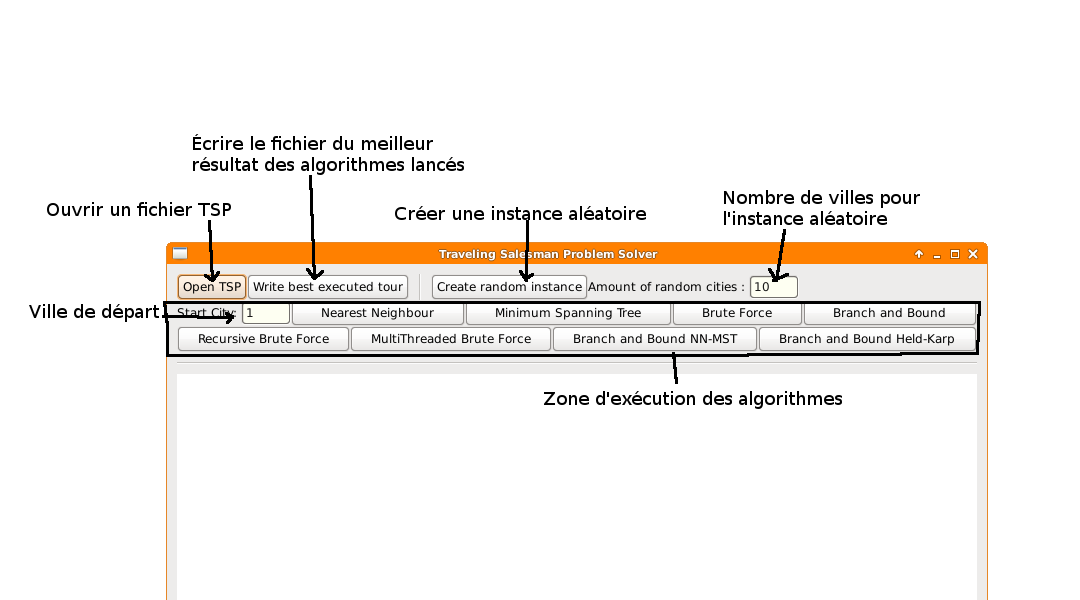
\includegraphics[width=\textwidth]{TSP_GUI.png} \\

Vous pouvez lancer le mode graphique avec un fichier préchargé en ajoutant le nom du fichier \\
\emph{./VDC -g fichier1.tsp}

\subsubsection[scale=0.4]{Charger une instance}

Cliquez sur "Open TSP" et choisissez le fichier TSPLIB à charger.

\subsubsection{Générer une instance aléatoire}

Remplissez l'entrée de texte "\textit{Amount of random Cities}" avec la taille de l'instance aléatoire que vous souhaitez générer. En suite, cliquer sur le bouton "\textit{Create Random Instance}".

\subsubsection{Lancer un algorithme}

Vous devez avoir ouvert une instance. Remplissez l'entrée de texte "Start City" avec un nombre entier compris entre 1 et la taille de l'instance chargée, puis cliquez sur un des boutons choisissant l'algorithme que vous souhaitez lancer.\\
Il est possible de sauvegarder le résultat de vos algorithmes au format \textbf{TSPLIB} (.tour) : Executez les algorithmes de votre choix puis cliquez sur "Write best executed tour", le programme selectionnera le résultat de l'algorithme ayant réalisé le plus court chemin et exportera le fichier.


\subsection{Mettre en route le site web TSP}

Pour que le site web PHP disponible dans le dossier \textbf{website/} fonctionne:\\
Il faut que le dossier \textbf{uploads/} soit en permission \textbf{777}.\\
Il faut que l'executable compilé soit dans le dossier \textbf{./}.\\
Avoir la fonction \textbf{shell\_exec} de \textbf{PHP} activée.


%----------------------------------------------------------------------------------------
%	CHAPITRE 3 ARCHITECTURE DU LOGICIEL 
%----------------------------------------------------------------------------------------

%3 Architecture
\chapter{Architecture du \textit{Traveling Salesman Problem Solver}}

%3.1 Résumé de l'architecture
\section{Introduction}


Nous avons défini le problème par une instance \textit{Map} qui contiendrait des instances \textit{City}. \\
Chaque instance City contient un tableau de distances relatives aux autres \textit{City} de la \textit{Map}, de plus elle contient un Point si ses coordonnées sont explicitées dans le fichier TSP. 
Un point est défini par ses coordonnées (x,y).\\

Pour faciliter l'implémentation du reste du programme et la compréhension du code, notamment des algorithmes, nous avez veillé à utiliser des \underline{prototypes de fonction facilement assimilables} et le plus explicite possible. Ainsi par exemple, les fonctions des modules \textit{City} et \textit{Map} contiennent toutes le préfixe associé à leur nature.
Nous avons bien entendu opté pour le choix de les nommer en anglais pour une question d'universalité.

L'exécution des algorithmes ainsi que leur implémentation sont faites dans le module \textit{Algos}. \\
Pour ouvrir, enregistrer les fichiers TSPLIB et exporter les résultats, un module \textit{TSP} a été réalisé.\\



%Optionnelles

Nous avons implémenté une interface graphique (\textit{GUI}) à l'aide de la librairie \textit{GTK+}.

Nous sommes allés plus loin avec le module API, qui sert à écrire le résultat dans fichier au format générique \textit{JSON}, qui est lisible et peut être facilement représenté et analysé dans n'importe quel langage de programmation.\\
Nous avons implémenté un petit site en \textit{PHP} qui exploite nos fichiers au format \textit{JSON}. \\



% MAIN
\section{\textit{main}}

La base du programme contient les fonctions d'usage, d'aide et de gestion d'options, il permet l'intéraction facilitée entre l'utilisateur et les fonctions implementées dans les autres modules. \\


%MODULE POINT
\section{Module \textit{point}}

Le module point sert à définir les City dans un repère cartésien, si \textbf{DISPLAY\_DATA\_SECTION} est dans le fichier d'instance. \\
Il sert aussi à calculer les distances entre deux points.

\subsection{Coordonnées}

Un point est défini par ses coordonnées cartésiennes, qui sont deux nombres de type double : x et y.

\subsection{Fonctions}

Les fonctions que nous avons définis sont : 
\begin{itemize}
	\item setLengthType(bool) qui défini le mode de calcul de distance
    \item lengthEuc(Point,Point) qui calcule et renvoie la distance \underline{euclidienne} entre deux points
    \item lengthMan(Point,Point) qui calcule et renvoie la distance de \underline{Manhattan} entre deux points
    \item length(Point,Point) qui renvoie la distance selon le mode défini
    \item pointGetX(Point) qui renvoie l'abscisse du Point
    \item pointGetY(Point) qui renvoie l'ordonnée du Point
    \item boolEquals(Point,Point) qui renvoie l'égalité de deux points
    \item point(double,double) qui crée et renvoie un point 
\end{itemize}

% MODULE CITY
\section{Module \textit{city}}

Une ville (\textit{City}) est définie par son tableau de distance avec les autres villes,  et par un \textit{Point} optionnellement.


\subsection{Tableau de distance \textit{dists}}

Le tableau de distances \textit{dists} est un tableau d'une dimension du même nombre de villes que la \textit{Map}.

\subsection{Position \textit{point}}

Si \textit{isPos}, la condition qui dit si la ville est définie aussi par un Point, est à VRAIE, alors la ville a un Point défini dans sa structure.

\subsection{Fonctions}

\begin{itemize}
	\item cityCreate instancie une "ville" caractérisée par sa position et sa distance avec les autres villes.
    \item cityDelete détruit une instance City
    \item cityGetDist qui permet d'obtenir la distance d'une \textit{City} avec une autre
    \item cityGetDistsSize retourne le nombre de distances que contient une \textit{City} c
    \item cityGetIsPos indique si un Point est défini par des coordonnées ou non.
    \item cityGetPos si cityGetIsPos est vraie, fournit les coordonnées de la \textit{City} (\textit{Point})
    \item cityEquals indique si 2 objets de type \textit{City} sont les mêmes. (comparaison des tableaux de distance)
    \item cityDataDump affiche toutes les informations connues sur une \textit{City}.
    \item cityGetIndice retourne l'indice de la \textit{City}.
\end{itemize}

% MODULE MAP
\section{Module \textit{map}}

La structure \textit{Map} est définie par un tableau de \textit{City}\\
La structure Map, étant une instance du problème, nous avons ajouté la sauvegarde des résultats à l'intérieur même de cette structure.

\subsection{Nom de l'instance \textit{name}}

Elle est définie par le nom du fichier instancié, ou de Random\_Map\_ si c'est une instance aléatoire.\\
Elle sert par exemple à nommer le nom du fichier de résultat.

\subsection{Tableau d'objets de type City \textit{cities}}

C'est un tableau extensible qui contient les villes de type City\\
On utilise nbCitiesMax pour connaître la taille max du tableau (pour la réallocation), ainsi que nbCities pour connaître la taille de l'instance.

\subsection{Sauvegarde des résultats}

Etant donné que Map est une instance de problème, nous avons besoin de sauvegarder les résultats dedans pour pouvoir sauvegarder la meilleure solution (le plus court chemin) calculée lors des appels d'un ou plusieurs algorithmes.


\subsubsection{Tableau de chemins \textit{paths}}
Prototype : City **paths\\
Un résultat est un chemin, un chemin est un tableau de City.\\
Nous utilisons le tableau de chemins pour pouvoir générer le fichier de résultat du meilleur algorithme lancé.\\
Il nous sert aussi dans l'interface graphique, pour ne pas recalculer des algorithmes déjà exécutés auparavant.
Paths contient un chemin pour chaque algorithme.

\subsubsection{Tableau de durées d'exécutions \textit{duration}}
Nous avons défini un tableau de réels (double) pour pouvoir sauvegarder les temps d'exécution des algorithmes avec leur chemin pour l'interface graphique. % et aussi pour l'écriture du fichier tour.

\subsection{Les fonctions}

Les fonctions implementeés pour intéragir avec la Map sont les suivantes  :
\begin{itemize}
	\item mapCreate() qui renvoie une Map vierge.
    \item mapGetName(Map) qui renvoie le nom de la Map.
    \item mapSetName(Map, Str) qui modifie le champ name de la Map.
    \item mapGetPath(Map, int) qui renvoie le tableau de City pour l'algorithme spécifié par son numéro.
    \item mapSetPath(Map, int, City *) qui modifie le champ paths[int] par celui passé en paramètre
    \item mapGetDuration(Map, int) qui renvoie la durée de calcul de l'algorithme spécifié par son numéro.
    \item mapSetDuration(Map, int, double) qui modifie la durée de calcul
    \item mapDelete(Map) qui supprime la Map
    \item mapDeleteRec(Map) qui supprime la Map et récursivement ses City.
    \item mapAddCity(Map,City) qui ajoute une ville à une Map
    \item mapGetCity(Map,int) qui renvoie une ville par son indice
    \item mapSetCity(Map,City, int) qui remplace une ville d'indice spécifié par une autre 
    \item mapGetSize(Map) qui renvoie la taille de l'instance (le nombre de City)
    \item mapGetIndiceCity(Map, City) qui renvoie l'indice de la City de la Map
    \item mapGetIsPos(Map) qui renvoie si les City de la map sont définis par des points
    \item mapDataDump(Map) qui affiche en mode verbeux tout le contenu de la Map
    \item mapCreateFromPoints(Point *, int , Str) crée une Map et ses villes en calculant les tableaux de distances à partir du tableau de Point
    \item mapCreateRandom(int) qui renvoie une Map créée aléatoirement avec le nombre spécifié de City
    \item  mapDraw(Map) dessine en mode textuel les points de la Map
\end{itemize}


%MODULE ALGOS
\section{Algorithmes}


\subsection{Nearest Neighbour}

\subsubsection{Présentation de Nearest Neighbour}

Le problème de la recherche des plus proches voisins \textit{Nearest Neighbour} (ou des k plus proches voisins) est très courante en algorithmique et de nombreux auteurs ont proposé des algorithmes efficaces pour le résoudre rapidement.\\

C’est un algorithme avec une heuristique simple, aussi appelé algorithme glouton, le principe est qu'il fait un choix à chaque étape, sans jamais remettre en cause ce choix.

Soient :
\begin{itemize}
    \item un espace E de dimension D ;
    \item un ensemble A de N points dans cet espace ;
    \item un entier k plus petit que N.
\end{itemize}
La recherche des plus proches voisins consiste, étant donné un point x de E n'appartenant pas nécessairement à A, à déterminer quels sont les k points de A les plus proches de x. On parle alors de trouver un voisinage de taille k autour du point x.


\subsubsection{Algorithme}

fonction nearestNeighbour \{


\indent pour i allant de 1 à k\\
\indent \indent mettre le point D[i] dans proches\_voisins\\
\indent fin pour\\
\indent pour i allant de k+1 à N\\
\indent \indent si la distance entre D[i] et x est inférieure à la distance d'un des points de proches\_voisins à x\\
\indent \indent \indent supprimer de proches\_voisins le point le plus éloigné de x\\
\indent \indent \indent mettre dans proches\_voisins le point D[i] \\
\indent \indent fin si\\
\indent fin pour\\
\indent proches\_voisins contient les k plus proches voisins de x\\
            
\indent\} \\

L'algorithme Nearest Neighbour a été implémenté en complexité de temps \(\theta(n^2)\)



\subsection{Minimum Spanning Tree}

\subsubsection{Présentation de Minimum Spanning Tree}

En théorie des graphes, étant donné un graphe non orienté connexe dont les arêtes sont pondérées, un arbre couvrant de poids minimal \textit{minimum spanning tree} de ce graphe est un arbre couvrant (sous-ensemble qui est un arbre et qui connecte tous les sommets ensemble) dont la somme des poids des arêtes est minimale. L'arbre couvrant de poids minimal est aussi connu sous certains autres noms, tel qu’arbre couvrant minimum ou encore arbre sous-tendant minimum.

\subsubsection{Implémentation de Minimum Spanning Tree}

\indent L'arbre couvrant de poids minimal est implémenté par une structure arbre sous forme de liste chaînée. Cette structure contient aussi un tableau des sommets de l'arbre pour un rajout de sommet plus facile. Le chemin est ensuite généré en parcourant cette arbre. \\

L'algorithme a été implementé avec une complexité de temps \(\theta(n^3)\) \\

\subsection{Recherche exhaustive \textit{BruteForce}}

La recherche exhaustive ou recherche par force brute est un terme qui s'applique à une catégorie de méta-algorithmes.\\
Elle calcule toutes les possibilités de chemins possible. \\
Soit une complexité de l'ordre \(\theta(n!)\) \\

\subsubsection{Version itérative}

Nous avons implementé une version itérative de Bruteforce, en effet, une version récursive est plus lente car elle utilise la pile d'exécution.\\

Nous utilisons un algorithme de Permutation non ordonnée \textit{QuickPerm}, du type :\\

\noindent fonction permutation(){ \\
\indent entier nombre ville N \\
\indent tableau d'entiers t[N] initialisé avec (1,2,..., N) , p[N] initialisé à 0 \\
\indent entier i, j, tmp \\
\indent i=1\\
\indent tantque(i<N)\\
\indent\indent si(p[i]<i)\\
\indent\indent\indent j=i\%2*p[i]\\
\indent\indent\indent tmp = a[j]\\
\indent\indent\indent a[j] = a[i]\\
\indent\indent\indent a[i] = tmp\\
\indent\indent\indent p[i]++\\
\indent\indent\indent // on calcule la distance à ce moment là\\
\indent\indent sinon\\
\indent\indent\indent p[i]=0\\
\indent\indent\indent i++\\
\indent\indent finsi \\
\indent fintantque\\
\}\\


    \begin{tabular}{|l|l|l|}
    \hline
    1 & 2 & 3 \\ \hline
    2 & 1 & 3 \\ \hline
    3 & 1 & 2 \\ \hline
    1 & 3 & 2 \\ \hline
    2 & 3 & 1 \\ \hline
    3 & 2 & 1 \\ \hline
    \end{tabular}\\
\textit{Exemple de permutations avec 1,2,3 \\}

\subsubsection{Version récursive}

La version récursive, est plus facile à implémenter, mais elle utilise la pile d'exécution. \\
Le plus dans cette méthode, c'est qu'elle fait les permutations ordinales. \\

L'algorithme de l'université d'Exeter a été implémenté. \\

fonction permutation(tableau de villes v, entier debut, entier n)
\{  \\
\indent si (debut == n-1) { \\
\indent \indent  // on a le chemin complet\\
\indent sinon {\\
\indent \indent pour (entier i = debut; i < n; i++) {\\
\indent \indent \indent entier tmp = v[i];\\
      
\indent \indent \indent v[i] = v[debut];\\
\indent \indent \indent v[debut] = tmp;\\
\indent \indent \indent permutation(v, debut+1, n);\\
\indent \indent \indent v[debut] = v[i];\\
\indent \indent \indent v[i] = tmp;\\
\indent \indent finpour\\
\indent finsi \\
\}

\subsubsection{Version multi-threadée}

Nous avons exprimé le besoin de paralleliser le bruteforce, pour peut être gagner un peu de temps. \\
Nous avons donc décomposé le problème d'une Map de N Cities, à N-1 sous-problème, que nous enverrons à un thread respectivement. \\


    \begin{tabular}{|l|l|l|l|l|}
    \hline
    1 (Ville de départ) & 2 & 3 & 4 & 5 \\ \hline
    Sous problème 1     & 2 & 3 & 4 & 5 \\ \hline
    Sous problème 2     & 3 & 2 & 4 & 5 \\ \hline
    Sous problème 3     & 4 & 2 & 4 & 5 \\ \hline
    Sous problème 4     & 5 & 2 & 3 & 4 \\ \hline
    \end{tabular}\\
   

   Cela, en pratique, nous diminue le temps (réel) par le nombre de threads lancé. \\
\subsection{Séparation et évaluation \textit{Branch and Bound}}

\subsubsection{Présentation}

Un algorithme par séparation et évaluation, également appelé selon le terme anglophone branch and bound, est une méthode générique de résolution de problèmes d'optimisation, et plus particulièrement d'optimisation combinatoire ou discrète. C'est une méthode d'énumération implicite : toutes les solutions possibles du problème peuvent être énumérées mais, l'analyse des propriétés du problème permet d'éviter l'énumération de larges classes de mauvaises solutions. Dans un bon algorithme par séparation et évaluation, seules les solutions potentiellement bonnes sont donc énumérées.

\subsubsection{Algorithme natif}

L'algorithme que nous avons implémenté est basé sur l'algorithme Bruteforce, version récursive. \\
Elle nous permettra de stopper la récursion dès que la distance de la branche déjà générée. \\

fonction permutation(tableau de villes v, entier debut, entier n)
\{  \\
\indent si (debut == n-1) { \\
\indent \indent  // on a le chemin complet\\
\indent\indent si (longueur(v)<pluspetitcheminactuel) \\
\indent\indent\indent pluspetitcheminactuel=longueur(v) \\
\indent\indent finsi\\
\indent sinon {\\
\indent \indent pour (entier i = debut; i < n; i++) {\\
\indent \indent \indent entier tmp = v[i];\\
      
\indent \indent \indent v[i] = v[debut];\\
\indent \indent \indent v[debut] = tmp;\\
\indent \indent \indent si (longueur(v) > pluspetitcheminactuel)\\
\indent\indent\indent\indent interruption\\
\indent\indent\indent finsi\\
\indent \indent \indent permutation(v, debut+1, n);\\
\indent \indent \indent v[debut] = v[i];\\
\indent \indent \indent v[i] = tmp;\\
\indent \indent finpour\\
\indent finsi \\
\}


\subsubsection{Algorithme relaxé avec Nearest Neighbour et Minimum Spanning Tree}

L'algorithme a juste une initialisation de plus petit chemin actuel (lower bound) au minimum des distances des résultats de Nearest Neighbour et Minimum Spanning Tree.

Nous avons décidé d'initialisé par les deux valeurs, car :
\begin{itemize}
\item Étant donné qu'en pratique (sur des instances variants de 10 à 100 villes) Nearest Neighbour donne des résultats plutôt meilleurs que Minimum Spanning Tree.
\item Minimum Spanning Tree donne un résultat maximum à deux fois l'optimal, du coup cela sera borné.
\end{itemize}

\subsubsection{Algorithme relaxé de Held Karp}

Pour toutes les arêtes e, avec w\textsubscript{e} la longueur de l'arête e, et la variable x\textsubscript{e} est à 1 si l'arête e est dans le tour, sinon 0. \
Pour tous les sous-ensembles S d'un sommet, \(\delta(S)\) définissent les arêtes connectants un sommet dans S avec un sommet extérieur à S.\\

\noindent 1. pour tous les sommets v, sommer\textsubscript{arêtes e dans \(\delta({v})\)} x\textsubscript{e} = 2 \\
2. pour tous les sous-ensembles non vides S de sommets, sommer\textsubscript{arêtes e dans \(\delta(S)\)} \\ x\textsubscript{e} >=2 \\
3. pour toutes les arêtes e dans E, x\textsubscript{e} appartient à \{0, 1\}\\

Il faut que l'ensemble des arêtes soit un groupement de tour (1), et qu'il n'y en a qu'une (2). \
(Sinon il faudra définir S comme étant un ensemble de sommets visités par un seul des tours).\\
3. pour toutes les arêtes e dans E, \(0 <= x\textsubscript{e} <= 1\) \\

Nous appliquons les optimisations des multiplicateurs de Lagrange, puis l'optimisation de l'algorithme du gradient.  \
Cela se résume à calculer un minimum spanning tree et en suite modifier certaines directions via le calcul de one-tree. \\

L'algorithme de \textit{Branch and Bound} a été implémenté via un tas Minimum de solutions partielles triées par la valeur de \textit{Held Karp} de ces solutions. \\

Soit \(h\) étant un tas min de solutions partielles, triée par \textit{Held-Karp} \\
soit \(meilleursolution\) = null \\
soit \(solactuelle\) la solution partielle de \textit{Held-Karp}\\

\indent tantque \(solactuelle\) n'est pas une solution complète et la valeur de \textit{Held-Karp} de \textit{solactuelle} est meilleure que \(meilleursolution\) \\
\indent \indent choisir un embranchement \(v\) \\
\indent \indent soit \(sol0\) la connexion avec solactuelle \(\{v -> 0\}\) \\
\indent \indent soit \(sol1\) la connexion avec solactuelle \(\{v -> 1\}\) \\
\indent \indent calculer \(sol0\) et \(sol1\) \\
\indent \indent soit \(solactuelle\) la meilleure des deux solutions \(sol0\) et \(sol1\); mettre la moins bonne dans le tas Min \(h\) \\
\indent fintantque\\
\indent si solactuelle est meilleure que meilleursolution alors\\
\indent soit meilleursolution = solactuelle \\
\indent supprimer tous les vertex du tas Min \(h\) ayant une valeur de HK pire que \(solactuelle\) \\
\indent finsi \\
\indent si \(h\) est vide alors arrêter; // nous avons trouver la solution optimale \\
\indent récupérer le sommet du tas Min \(h\) et le mettre dans \(solactuelle\)


%MODULE TSP
\section{Module \textit{tsp}}

Il nous a été demandé d'implémenter un lecteur de fichiers TSP au format TSPLIB.

\begin{itemize}
\item Map tspLoad(filename) => Prend un nom de fichier en paramètre et retourne un objet Map
\item void tspWrite(Map, Str) => Prend un objet Map et un nom de fichier en paramètre et écrit le fichier résultant
\item void tspOut(Map, City*, Str, Str) => Prend une Map, un parcours, un nom de fichier et un commentaire en paramètre et écrit le résultat dans le fichier
\end{itemize}

\subsection{Module \textit{string}}

C'est une librairie qu'a écrit Jason pour un autre projet, elle décrit des fonctions de gestion des chaines de caractères plus évoluées que celles prévues de base, comme par exemple indexOf(), fonction native en JAVA.

\subsection{Ouverture de fichiers TSPLIB}

Le fichier est lu ligne par ligne et sauvegarde les informations petit à petit, si tout s'est bien passé en fin de lecture il crée un objet Map qu'il remplit avec les City nécessaires et le renvoie, prêt à l'emploi.
Le lecteur est capable de lire des fichier TSP qui ne comportent pas de DISPLAY\_DATA\_SECTION, dans ce cas il n'y aura pas d'affichage possible, à l'inverse le lecteur lit les fichiers qui ont le DISPLAY\_DATA\_SECTION mais pas le EDGE\_WEIGHT\_SECTION, dans ce cas le lecteur va calculer les distances automatiquement selon le mode choisi avec les options (Manhattan par défaut) et retournera une Map conforme à l'emploi. Ex d'utilisation : \textit{./VDC -nn toto.tsp}

\subsection{Sauvegarde de fichiers TSPLIB}

C'est la fonction inverse de la lecture, à partir d'une Map la fonction va générer un fichier TSP, cette fonctionnalité est utilisé pour rendre des TSP à partir de maps aléatoires. Ex d'utilisation : \textit{./VDC -r 10 -o toto.tsp}

\subsection{Sauvegarde des résultats au format TSPLIB}

Cette fonction sert a rendre des fichiers TSP TOUR, c'est-à-dire des chemins à parcourir selon les résultats d'un ou plusieurs algorithmes à partir d'une Map, d'une liste de villes, d'un nom de fichier et d'un commentaire.Ex d'utilisation : \textit{./VDC toto.tsp -all -to}


%MODULE COMPLEMENTAIRES AUX ALGORITHMES
\section{Module \textit{tree}, \textit{vertex}, \textit{File de priorité \textit{pri\_queue}}}

Nous avons du implémenter des modules complémentaires à notre structure de base pour permettre l'implémentation de certains algorithmes.

\subsection{tree}

C'est un module qui permet de créer un arbre planaire et de le parcourir. \
Il a été implémenté pour l'algorithme Minimum Spanning Tree. \
Nous avons un accès au père et aux fils. \
Il contient aussi un tableau avec toutes les adresses des sommets dans l'arbre. \

\subsection{vertex}

C'est un module qui implémente un vertex (sommet). Nous l'avons implémenté pour l'algorithme de branch and Bound. \
Il permet entre autres : 
\begin{itemize}
\item d'accéder au tableau d'exclusions d'arêtes
\item d'accéder à la distance ajustée
\item d'accéder au lower bound (la distance minimale)
\item d'accéder au degré
\item d'accéder au parent
\end{itemize}

\subsection{priority queue}

C'est un module d'implémentation d'une file de priorité. \
Elle nous permet de l'utiliser en tant que tas min. \
On peut entre autres : 
\begin{itemize}
\item ajouter un vertex au tas min
\item connaître la valeur du tas min
\item enlever le sommet du tas min
\item combiner deux tas min
\end{itemize}

%MODULE API 
\section{Fichier de sortie d'une instance au format JSON (API)}

Nous avons eu l'idée de rendre les traitements de notre programme disponibles dans un format facile à comprendre et à analyser syntaxiquement.\\
C'est pour cela que nous avons mis une option -api, qui va sortir un fichier au format JSON pour chaque algorithme différent.

\subsection{Format JSON}

\textbf{JSON} (JavaScript Object Notation – Notation Objet issue de JavaScript) est un format léger d'échange de données. Il est facile à lire ou à écrire pour des humains. Il est aisément analysable ou générable par des machines. Ces propriétés font de JSON un langage d'échange de données idéal.

\subsection{Sortie des fichiers JSON}

Les données sorties sont les traitements (nom, matrice de distance, positions s'il y a, chemins (par indice), tableau de distances (entre deux villes), le nom de l'algorithme.\\
Les noms des fichiers sorties selon les algorithmes sont les noms des fichiers d'entrées avec le suffixe de l'option d'algorithme appelé, rajoutez à cela .json. \\
Par exemple : \\
<NomFichier>\_nn.json  pour l'algorithme Nearest Neighbour.\\
<NomFichier>\_mst.json  pour l'algorithme Minimum Spanning Tree.\\
<NomFichier>\_opt.json  pour l'algorithme Branch and Bound avec relaxation de Held Karp.


\subsection{Implémentation dans un site web}

Il est possible de résoudre des problèmes (de petites instances pour des raisons de performances) via un site web, où l'utilisateur peut envoyer un fichier TSP (que notre programme peut lire, soit FULL\_MATRIX).\\
L'implémentation est disponible en ligne sur \url{http://david.phan.emi.u-bordeaux1.fr/S4/EDD/API_WEB_TSP/}. Nous utilisons la bibliothèque Javascript Graph Dracula pour afficher les instances.

\subsection{Analyse des données JSON}

La récupération des données du programme étant facilité, avec des fonctions PHP json\_decode, nous avons récupéré les résultats de lectures, et d'algorithmes facilement. (disponible dans le fichier \textit{libjson.php})

\subsection{Fonctions}

\begin{itemize}
	\item executeApis(Map, bool*, int, char *) qui execute les algorithmes avec la Map donnée en paramètre et les algorithmes choisis
    \item printJSON(Map,City *, int, char*) écrit le fichier JSON
\end{itemize}




%----------------------------------------------------------------------------------------
%	CHAPITRE 4 TESTS ET PERFORMANCES
%----------------------------------------------------------------------------------------
\chapter{Tests et performances}

%TESTS

\section{Tests}

\subsection{Tests du lecteur de TSP}

Nous avons effectué des tests basiques qui consistent à lire les fichiers TSP avec le programme, puis de le comparer à ce que voyons dans le fichier TSPLIB. Ce genre de tests est très limité (pour de grandes instances).\\
Par la suite, pour automatiser la vérification du lecteur de TSP, nous avons créé un \textit{CTest} automatisé qui nous permet de lancer la lecture de fichiers connus exemple10.tsp exemple14.tsp bays29.tsp et de les analyser et comparer avec les résultats précédents (vérifiés par nos soins).

\subsection{Tests de fichiers TSP fournis}

Nous avons lancé les différents algorithmes sur les instances, et comparés les résultats (longueur) de celles ci avec les optimales fournies.\

    \begin{tabular}{|l|l|l|l|l|l|l|}
    \hline
    ~   & exemple10 & exemple14 & bays29 & spanning30 & ch130.      & pr1002        \\ \hline
    NN  & 46        & 38.688102 & 2258   & 60.004190  & 7575.285301 & 315596.596000 \\ \hline
    MST & 52        & 34.962292 & 2423   & 60.004190  & 8128.755901 & 351387.186000 \\ \hline
    OPT & 42        & 30.878491 & 2020   & 60.004190  & 6110        & 259045        \\ \hline
    \end{tabular}\\


    Comme nous pouvons le voir, la longueur résultante de Minimum Spanning Tree est toujours inférieur à 2 fois la longueur optimale.
    
\subsection{Tests d'instances générées}

L'option "\textit{-}r" vue en exemple précédemment permet d'effectuer des tests sur des matrices de point aléatoire, en spécifiant le nombre de villes voulu, la fonction main va faire appel à la fonction \textbf{mapCreateRandom} du module \textit{Map}, le fonctionnement de cette dernière est le suivant :
\begin{itemize}
	\item création d'un tableau de \textit{Point} de taille le nombre de villes spécifié
    \item initialisation des champs x et y du tableau à une valeur aléatoire comprise entre 0 et 1000
    \item initialisation du nom de la fonction
    \item appel à la fonction \textbf{mapCreateFromPoints} qui instancie la map et la remplit avec le tableau de \textit{Point}
\end{itemize}


\section{Performances}

Pour nos tests de performances, nous avons lancé nos instances sur des ordinateurs de même configuration technique, \textit{infini1 infini2 infini3 infini4}.

\subsection{Nearest Neighbour}

\begin{tikzpicture}
\begin{axis}[
height=8cm,width=12cm
,axis x line=bottom,axis y line=left
,xmin=0,xmax=3.12
,ymin=0,ymax=5.89472
,title={}
,xlabel={10${^3}$ villes}
,ylabel={10${^3}$ ms}
]
\addplot[draw=blue
,mark=none,smooth
] file
 {nn.txt};
\end{axis}
\end{tikzpicture}
\newline

\begin{tabular}{|l|l|l|l|l|l|l|l|l|l|}
    \hline
    Taille de l'instance  & 100   & 200   & 300   & 400   & 500   & 800  & 1000  & 2000 & 3000 \\ \hline
    Nearest Neighbour (s) & 0.001 & 0.003 & 0.008 & 0.017 & 0.032 & 0.123 & 0.233 &  1.744 & 5.668  \\ \hline
\end{tabular}

\subsection{Minimum Spanning Tree}

\begin{tikzpicture}
\begin{axis}[
height=8cm,width=12cm
,axis x line=bottom,axis y line=left
,xmin=0,xmax=1.04
,ymin=0,ymax=140.06824
,title={}
,xlabel={nbvilles/10${^3}$ villes}
,ylabel={MST/10${^3}$ ms}
]
\addplot[draw=blue
,mark=none,smooth
] file
 {mst.txt};
\end{axis}
\end{tikzpicture}

\begin{tabular}{|l|l|l|l|l|l|l|l|}
    \hline
    Taille de l'instance  & 100  & 200 & 300 & 400 & 500 & 800 & 1000 \\ \hline
    Temps d'exécution(s) & 0.023 & 0.296 & 1.326 & 3.800 & 9.011 & 55.80 & 134.7 \\ \hline
\end{tabular}


\subsection{BruteForce}

\begin{tikzpicture}
\begin{axis}[
height=8cm,width=12cm
,axis x line=bottom,axis y line=left
,xmin=10,xmax=13
,ymin=0,ymax=107.54224
,title={}
,xlabel={villes}
,ylabel={10${^3}$ ms}
]
\addplot[draw=blue
,mark=none,smooth
] file
 {bf1.txt};
\addplot[draw=red
,mark=none,smooth
] file
 {bf2.txt};
\addplot[draw=green
,mark=none,smooth
] file
 {bf3.txt};
\end{axis}
\end{tikzpicture}
\newline
Bleu : BF itératif
\newline
Rouge : BF récursif
\newline
Vert : BF multithread
\newline


\subsubsection{BruteForce Iteratif}


\begin{tabular}{|l|l|l|l|l|l|l|l|}
	\hline 
	 Taille de l'instance &exemple10 &11 &12 &13 &exemple14  \\ \hline
     Temps d'exécution(ms) &32.1 &349 &4096 &47856 &654195 \\ \hline
\end{tabular}
\vspace{1cm}

\subsubsection{BruteForce Multi-threadé}

\begin{tabular}{|l|l|l|l|l|l|l|l|}
	\hline 
	 Taille de l'instance &exemple10 &11 &12 &13 &exemple14  \\ \hline
 	 Temps d'exécution(ms) &90 &808 &24441 &382495 &138881517 \\ \hline
     Temps réel(ms) & 18 &119 &2521 & 37772 & 1142940\\ \hline
\end{tabular} \\
\newline

La version multithreadé n'est pas très performante comme nous pouvons le voir. \
Le fait d'avoir un problème parallelisable ne nous signifie pas qu'on peut gagner des performances.

\subsubsection{BruteForce Récursif}
\begin{tabular}{|l|l|l|l|l|l|l|l|}
	\hline 
    Taille de l'instance &exemple10 &11 &12 &13 &exemple14  \\ \hline
    Temps d'exécution(ms) &58.1 &638.6 &7750.3 &99740 &1385947 \\ \hline
\end{tabular}\\
\newline
Il est clair d'après les tableaux et le graphique que le BruteForce itératif est le plus efficace des trois versions (environ 10 minutes pour 14 villes). Cependant, à partir de 15 villes (inclues) il n'est pas la peine d'essayer de résoudre un tsp avec un algorithme de BruteForce, cela prendrait beaucoup trop de temps.


\subsection{Branch and Bound}

\begin{tabular}{|l|l|l|l|l|l|l|l|}
	\hline 
	 Taille de l'instance &exemple10 &12 &exemple14 &16 \\ \hline
     Branch and Bound &6.356 &40-300 & 6707 &23884\\ \hline
     B\&BR(nn-mst) &6 &40-300 &6685 &16483\\ \hline
     B\&BRHK &0.036 &0.058 &0.115 &0.225\\ \hline
     
\end{tabular}

\subsubsection{Branch and Bound}

Pour la relaxation de Held-Karp uniquement, il est possible de résoudre des problème une centaine de villes, mais la rapidité varie énormément selon l'instance, en effet cela dépend du calcul du \textit{lower Bound} initial qui peut nous donner le pire des cas de \(\theta(2^n*n^2)\). En revanche on peut clairement dire que celui-ci est le plus optimisé et donne les meilleurs résultats. Cela peut aussi s'expliquer par l'implémentation non récursive de Branch and Bound.

\subsubsection{Branch and Bound avec relaxation NN-MST}

\begin{tikzpicture}
\begin{axis}[
height=8cm,width=12cm
,axis x line=bottom,axis y line=left
,xmin=0,xmax=17.68
,ymin=0,ymax=77.20232
,title={}
,xlabel={villes}
,ylabel={10${^3}$ ms}
]
\addplot[draw=blue
,mark=none,smooth
] file
 {bb1.txt};
\addplot[draw=red
,mark=none,smooth
] file
 {bb2.txt};
\end{axis}
\end{tikzpicture}
\newline
Bleu : BB classique
\newline
Rouge : BB relaxé NN-MST
\newline

On constate une légère amélioration du BB classique qu'on a encore plus creusé avec la relaxation de Held-Karp.

\subsubsection{Branch and Bound avec relaxation de Held-Karp}

\begin{tikzpicture}
\begin{axis}[
height=8cm,width=12cm
,axis x line=bottom,axis y line=left
,xmin=0,xmax=88.4
,ymin=0,ymax=19.084
,title={}
,xlabel={villes}
,ylabel={10${^3}$ ms}
]
\addplot[draw=blue
,mark=none,smooth
] file
 {bbhk.txt};
\end{axis}
\end{tikzpicture}

Ce graphe montre bien la non linéarité de l'algorithme. En effet, le temps d'exécution dépend de l'organisation profitable ou non des villes. Cela s'explique avec le calcul du \textit{lowerBound}, et donc de la séparation des possibilités.


%----------------------------------------------------------------------------------------
%	CHAPITRE 5 ORGANISATION ET REPARTITIONS
%----------------------------------------------------------------------------------------

\chapter{Organisation du travail, répartition des tâches, utilisation des outils, et difficultés rencontrées}

\section{Organisation du travail}

\subsection{Premiers pas réflexion sur le découpage modulaire, premier algorithme}

Au départ, n'ayant pas connaissance des fichiers TSP, nous avons opté pour une implémentation résident sur des points décrivant la position de nos villes et une utilisation des calculs de longueurs pour éxecuter nos algorithmes. Dés le départ nous avons donc créé le type Point, City (les coordonnées) et Map (Une liste de City).

Nous avons commencé à implémenter Nearest Neighbour mais nous avons eu un problème, au lieu de rentrer manuellement la Map ou de coder le TSP reader tout d'abord, nous avons pensé à faire des Maps aléatoires de tailles données pour pouvoir ensuite vérifier les résultats. Par la suite nous avons gardé la fonctionnalité de Map aléatoires qui s'est avérée très utile.

\subsubsection{Découpage modulaire}

Par la suite, ayant pris connaissance de la structure des fichiers TSP et du fonctionnement du calcul des algorithmes, nous avons décidé que City contiendrait en plus un tableau de distances de la longueur du nombres de villes que contient la Map, ainsi chaque City contient les distances entre elle-même et les autres villes.

Les modules suivants s'ajoutent au programme :
\begin{itemize}
\item Api => Gestion de la sortie au format JSON
\item Fcts => Fonctions globales a plusieurs fichiers pour le fonctionnement du programme
\item Pri\_queue => Objet file de priorité
\item String => Librairie de gestion des chaines de caractères
\item Tsp => Librairie de gestion des fichiers TSP
\item Algos => Gestion de l'execution des algorithmes, coeur du programme 
\item Tree => Objet arbre planaire pour MST
\item Vertex => Objet arbre planaire pour BBHK
\item Gui => Gestion des tampons pour l'affichage
\item Guisys => Gestion de l'interface graphique
\end{itemize}


\subsection{Implémentations de tests, Automatisation des tests}

\subsubsection{Implémentations des tests}

\paragraph{Tests de fichiers fournis} \

Nous avons implémenté des tests automatisés avec CTest, qui lancent quelques algorithmes et vérifient les résultats mis en mémoire via les correspondances d'expressions régulières de nos chemins. \
De plus nous avons ajoutés des tests de lecture de TSP en vérifiant via des vérifications de châines de caractères.

\paragraph{Tests de performances automatisés} \

Nous avons implémenter une option pour lancer des batteries de tests sur des instances aléatoires avec l'option -t <nbTests> <nbVilles> commençant par 3 villes puis en allant jusqu'à <nbVilles>. \
Cela pour avoir des temps d'exécution.

\subsubsection{Fuites de mémoires}

Nous avons analysé avec Valgrind et supprimé au maximum les fuites de mémoires.
GTK+ provoque le reste des fuites mémoires.

\subsubsection{Analyse de complexité de Nearest Neighbour et Minimum Spanning Tree}

\paragraph{Complexité de Nearest Neighbour}

Le fait que nous avons implémenter l'algorithme Nearest Neighbour avec deux boucles imbriquées, nous indiquent que la complexité est de l'ordre de \(\theta(n^2)\)

\paragraph{Complexité de Minimum Spanning Tree}

Nous avons trois boucles implémentés dans notre implémentation. \
La complexité est dans l'ordre de \(\theta(n^3)\)

\subsection{Nouvelles versions de Bruteforce et de Branch and Bound}

\subsubsection{Nouvelles versions de Bruteforce}

Nous avons rajouté une version récursive pour pouvoir faire des tests de performances, le fait est, qu'une fonction récursive utilise la pile d'exécution et ne permet donc pas d'avoir de meilleures performances que la version itérative. \ 
Par contre l'algorithme utilisé nous génère des permutations ordonnées.

\subsubsection{Nouvelle version de Branch and Bound}

Nous avons implémenté une version sûre de Branch and Bound qui ne rentrera pas dans les mauvaises branches vu que nous arrêterons la récursion. \\
Puis nous avons ajouté une relaxation à cette version, c'est-à-dire d'initialiser le chemin minimal actuel à celui du chemin le plus court trouvé par Nearest Neighbour et Minimum Spanning Tree. \\
Nous avons en suite cherché un algorithme efficace sur internet, nous avons trouvé celui de Held-Karp qui fait une relaxation très bonne, et une implémentation de Branch and Bound avec un tas min.

\subsection{Ajouts de fonctions, modification de la structure, amélioration de l'interface graphique}

\subsubsection{Ajouts de fonctions}

\paragraph{Fonction d'écriture de résultat tspOut}

La fonction tspOut écrit le fichier .tour (au format TSPLIB) avec le meilleur résultat obtenu des algorithmes lancés.

\paragraph{Amélioration de l'interface graphique}

Nous avons ajouté la possibilité d'ouvrir un fichier depuis l'interface graphique, et donc de la rendre indépendante et facile d'utilisation. (Lancement avec un simple \textbf{./VDC -g} ) \\
Nous avons ajouté la possibilité de sauvegarder le meilleur tour, la possibilité de générer une instance aléatoire, la possibilité de définir la ville de départ.

\paragraph{Fonction d'écriture de résultat en format JSON}

Nous avons ajouté une fonction d'écriture du traitement et des résultats des algorithmes. Cela permettrait à un utilisateur qui voudrait, par exemple utiliser les données traitées par notre programme en détail.

\paragraph{Petit site web utilisant le format JSON}

Par exemple, nous avons implémenté un petit site écrit en PHP, utilisant des modules Javascript pour le dessin des graphes. Il permet au visiteur de la page d'envoyer son fichier TSPLIB, de choisir l'algorithme à lancer, puis de voir le résultat.

\paragraph{Ecriture du rapport}

Nous avons écrit le rapport avec LaTex et l'avons exporté en pdf.



\section{Utilisation des outils}

\subsection{Utilisation de Subversion}

Nous avons utilisé SVN avec Savane pour versionner notre projet et travailler à plusieurs, le stockage distant des données nous a aussi permis de travailler aussi bien au CREMI que chez nous.

\subsection{Utilisation de Code::Blocks}

Nous n'avons pas (ou très peu) utilisé emacs pour développer et avons préféré Code::Blocks, un IDE pour le C/C++ qui a de nombreuses fonctions facilitant le développement comme l'auto-complétion, la compilation et le Debug intégré... Code::Blocks fonctionne un peu comme Eclipse


\subsection{Makefile}

Nous avons choisi de faire un Makefile pour la compilation de notre projet, il est récursif et éxecute les Makefile des dossiers gui et algos, les options disponibles sont clean, cleanAll et doc qui respectivement suppriment tous les .o (fichiers objet), suppriment tous les .o et l'éxecutable, crée la documentation. Tous les fichiers Makefile ont leur double Makefile.db a éxecuter avec l'option make -f Makefile.db et qui compilent avec l'option -g de gcc soit la version Debug, a l'inverse les Makefile principaux compilent avec une optimisation maximum du code soit l'option -O3 de gcc


\subsection{Documentation du code par DOxygen}

\subsubsection{Documentation du code par DOxygen}

Doxygen est un générateur de documentation sous licence libre capable de produire une documentation logicielle à partir du code source d'un programme. Pour cela, il tient compte de la grammaire du langage dans lequel est écrit le code source, ainsi que des commentaires s'ils sont écrits dans un format particulier. \\
Nous avons commencé à commenter les fichiers .h et .c de plusieurs fichiers sources. 



\section{Répartitions des tâches et difficultés rencontrées}

\subsection{Répartitions des tâches}

\subsubsection{Travail collectif}

Nous nous sommes accordés sur le découpage modulaire.

Nous avons débogué les modules des uns et des autres.

Nous avons tous participé aux tests et fait la documentation.

\subsubsection{Tâches séparées}

\begin{itemize}
\item Raphaël Afanyan : Algos BB Held Karp, structures de données(File prio, vertex), 1e Makefile
\item Nicolas Marcy : Algorithme MST, tree.c, Les tests (prog+ctest), 2e Makefile
\item David Phan : Algos Brute Force (toutes versions), Branch and Bound (toutes versions, Held Karp avec Raphael), Api + Site Web, Amélioration GUI, implémentation test TSP Reader (CTest)
\item Jason Pindat : Structures de données (Point, City et Map), Gestionnaire d'execution des algos + gestionnaire d'erreurs + gestionnaire d'options du Main, Nearest Neighbour, TSP Reader, GUI, 3e Makefile
\end{itemize}


\subsection{Difficultés rencontrées}

Nous avons eu des problèmes avec SVN qui nous a supprimé des fichiers à certains moments et qui a fait des Merge automatique en supprimant du code qui aurait dû créer des conflits.


Le choix de la bibliothèque graphique pour la GUI et l'implémentation de cette dernière avec GTK+ a été difficile par moments.

Les Makefile à plusieurs reprises n'ont pas réagi comme nous l'avions prévu, la récursivité de ceux-ci et la mise en place des dépendances automatiques n'ont pas été les plus simples.


\chapter{Conclusion}

Pour clore ce rapport, nous voulions exprimer le fait que nous avons pris chacun beaucoup de plaisir à réaliser ce projet tous ensemble, pouvoir travailler en groupe de plus de 2, de plus avec des gens que nous apprécions a été quelque chose de nouveau et de très plaisant, la communication était très bonne, l'état d'esprit également. Nous sommes satisfaits du programme que nous avons produit, tout ce que nous avions en tête à l'origine a été réalisé, d'autres fonctionnalités auxquelles nous n'avions pas pensé sont venues au fur et à mesure et nous avons été capable de les implémenter. Grâce à cela, nous nous sentons désormais beaucoup plus à l'aise dans le langage C et dans la gestion de projet. Au final, nous remercions grandement notre professeur Irène DURAND pour nous avoir guidé sur la bonne voie tout au long du projet, ses conseils pour l'améliorer et ses suggestions qui ont poussé notre réflexion plus loin et nous ont permis de pouvoir réaliser plus de tâches.
\newpage

\end{document}